%%%%%%%%%%%%%%%%%%%%%%%%%%%%%%%%%%%%%%%%%
% Structured General Purpose Assignment
% LaTeX Template
%
% Template Name: Anthony
% The template was named after my friend Anthony.
% Strong inspired by Apache Hadoop and Java (programming language)
%
% Author: Ang LEE
%
% Blog: http://angli.me/
%
% Github: https://github.com/leeang/
%
%%%%%%%%%%%%%%%%%%%%%%%%%%%%%%%%%%%%%%%%%

%----------------------------------------------------------------------------------------
%	CONSTANTS
%----------------------------------------------------------------------------------------

\newcommand{\hmwkTitle}{Report\ \#2 A}					% Assignment title
\newcommand{\hmwkClass}{Signal Processing}				% Course name
\newcommand{\hmwkClassTime}{}							% Workshop time
\newcommand{\hmwkClassInstructor}{}						% Tutor name
\newcommand{\hmwkAuthorName}{Ang LEE}					% Student name

\newcommand{\hmwkGraphicsPath}{img/}					% Graphics path
\newcommand{\hmwkCodePath}{code/}						% Code path

%----------------------------------------------------------------------------------------
%	TEMPLATE
%----------------------------------------------------------------------------------------

\documentclass{article}

\usepackage{fancyhdr}	% Required for custom headers
\usepackage{lastpage}	% Required to determine the last page for the footer
\usepackage{extramarks} % Required for headers and footers
\usepackage{graphicx}	% Required to insert images
\graphicspath{\hmwkGraphicsPath}
\usepackage{lipsum} 	% Used for inserting dummy 'Lorem ipsum' text into the template

\usepackage{float}
\usepackage{epstopdf}	% Required to insert .eps images
\usepackage{amssymb}
\usepackage{amsmath}
\usepackage[hidelinks]{hyperref}

% MATLAB syntax highlighting
\usepackage{color}		% Required to define colors
\definecolor{commentColor}{RGB}{34,139,34}
\definecolor{stringColor}{RGB}{160,32,240}
\usepackage{listings}
\lstset{
	inputpath=\hmwkCodePath,
	language=Matlab,
	basicstyle=\footnotesize\ttfamily,
	keywordstyle=\color{blue},
	stringstyle=\color{stringColor},
	commentstyle=\usefont{T1}{pcr}{m}{n}\color{commentColor},
	breaklines=true,
	showstringspaces=false
}

% Margins
\topmargin=-0.45in
\evensidemargin=0in
\oddsidemargin=0in
\textwidth=6.5in
\textheight=9.0in
\headsep=0.25in

\linespread{1.1}		% Line spacing

% Set up the header and footer
\pagestyle{fancy}
\lhead{\hmwkTitle} % Header Left 
\chead{\hmwkAuthorName} % Header Center
\rhead{\hmwkClass} % Header Right
\lfoot{\url{https://github.com/leeang/Signal-Processing}} % Footer Left
\cfoot{} % Footer Center
\rfoot{Page\ \thepage\ of\ \pageref{LastPage}} % Footer Right
\renewcommand\headrulewidth{0.4pt} % Size of the header rule
\renewcommand\footrulewidth{0.4pt} % Size of the footer rule

\setlength\parindent{0pt} % Removes all indentation from paragraphs

%----------------------------------------------------------------------------------------
%	Problem and Section
%----------------------------------------------------------------------------------------

\newenvironment{homeworkProblem}[1]{
	\section*{#1}
	}{
}
\newenvironment{homeworkSection}[1]{
	\subsection*{#1}
	}{
}
\newcommand{\problemAnswer}[1]{
	\noindent\framebox[\columnwidth][c]{
		\begin{minipage}{0.98\columnwidth}
			#1
		\end{minipage}
	}
}

%----------------------------------------------------------------------------------------
%	Document
%----------------------------------------------------------------------------------------

\begin{document}

\newpage

%----------------------------------------------------------------------------------------
%	PROBLEM 1
%----------------------------------------------------------------------------------------

\begin{homeworkProblem}{Question 1}

\begin{homeworkSection}{a)}

\subsubsection*{(i)}
The z-transform of a discrete-time signal $x[n]$ is defined as 
\begin{equation}\label{A11}
H(z)=\sum_{n=-\infty}^{\infty}h[n]z^{-n}
\end{equation}
Where z is a complex variable. Set $z=e^{j\omega}$ and substitute into Eq. \ref{A11}, yields
\begin{align*}
H(e^{j\omega})&=\sum_{n=-\infty}^{\infty}h[n]e^{-j\omega n}\\
&=\cdots h[-2]e^{j2\omega}+h[-1]e^{j\omega}+h[0]e^{j\omega 0}+h[1]e^{-j\omega}+h[2]e^{-j2\omega}\cdots\\
\end{align*}
Apply time shift property to find out the time domain representation 
\begin{equation*}
h[n]=\cdots h[-2]\delta[n+2]+h[-1]\delta[n+1]+h[0]\delta[n]+h[1]\delta[n-1]+ h[2]\delta[n-2]\cdots\\
\end{equation*}
Now, if we set the complex variable $z_1=z^D=e^{j\omega D}$. Then 
\begin{align*}
H(e^{j\omega D})&=\sum_{n=-\infty}^{\infty}h[n]e^{-j\omega nD}\\
&=\cdots h[-2]e^{j2\omega D}+h[-1]e^{j\omega D}+h[0]e^{j\omega 0 D}+h[1]e^{-j\omega D}+h[2]e^{-j2\omega D}\cdots\\
\end{align*}
Convert it into time domain,
\begin{equation*}
h[n]=\cdots h[-2]\delta[n+2D]+h[-1]\delta[n+D]+h[0]\delta[n]+h[1]\delta[n-D]+h[2]\delta[n-2D]\cdots\\
\end{equation*}
\textbf{Obviously, the time domain signal has horizontally stretched out $D$ times.}

\subsubsection*{(ii)}
Comparing $H(e^{j\omega})$ and $H(e^{j\omega D})$, it is clear that the x-axis variable $\omega$ becomes $D\omega$, which means the spectrum in frequency domain has shrunk by $D$ times.

\end{homeworkSection}

\begin{homeworkSection}{b)}

Prior to answering (i), (ii) and (iii), we firstly sketch the magnitude response of $H(z)$ and $H(-z)$.

\begin{equation}
H(-z) = H(-e^{j\omega}) = H((-1) e^{j\omega}) = H(e^{j\pi} e^{j\omega}) = H(e^{j(\omega+\pi)})
\end{equation}

\begin{figure}[H]
\begin{minipage}[t]{0.5\linewidth}
\centering
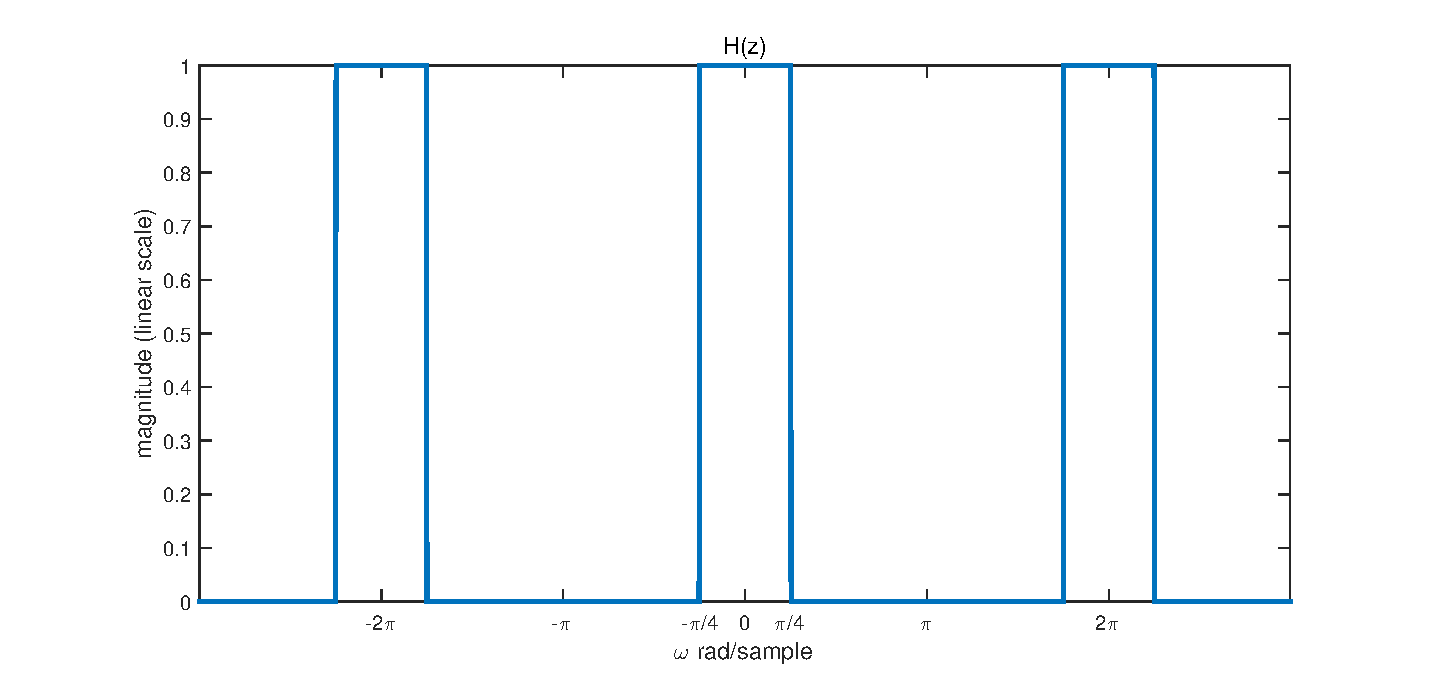
\includegraphics[width=3.3in]{A1b1.eps}
\caption{Magnitude response of $H(z)$}
\label{A1b1}
\end{minipage}
\begin{minipage}[t]{0.5\linewidth}
\centering
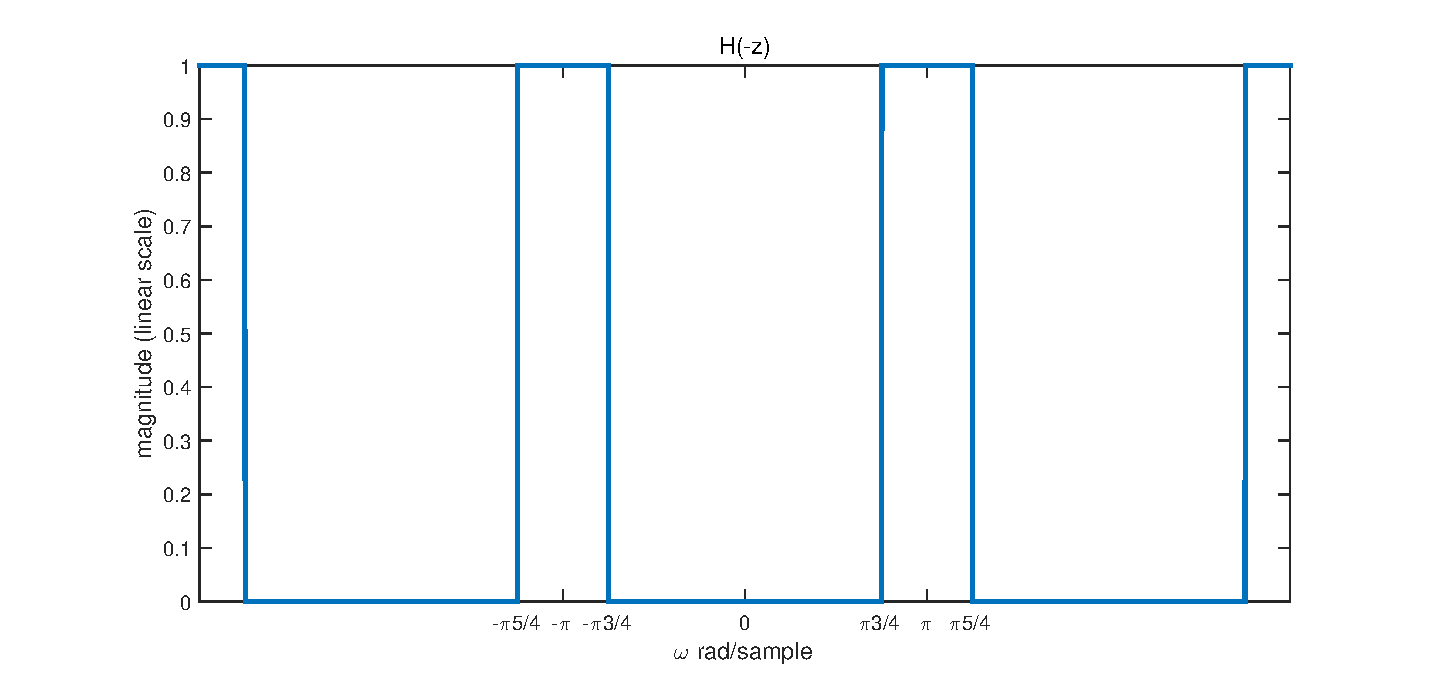
\includegraphics[width=3.3in]{A1b2.eps}
\caption{Magnitude response of $H(-z)$}
\label{A1b2}
\end{minipage}
\end{figure}

\subsubsection*{(i)}
Using the conclusion from Question 1(i), when $z\rightarrow z^3$, the spectrum will shrink by a factor of 3.

\begin{figure}[H]
\centering
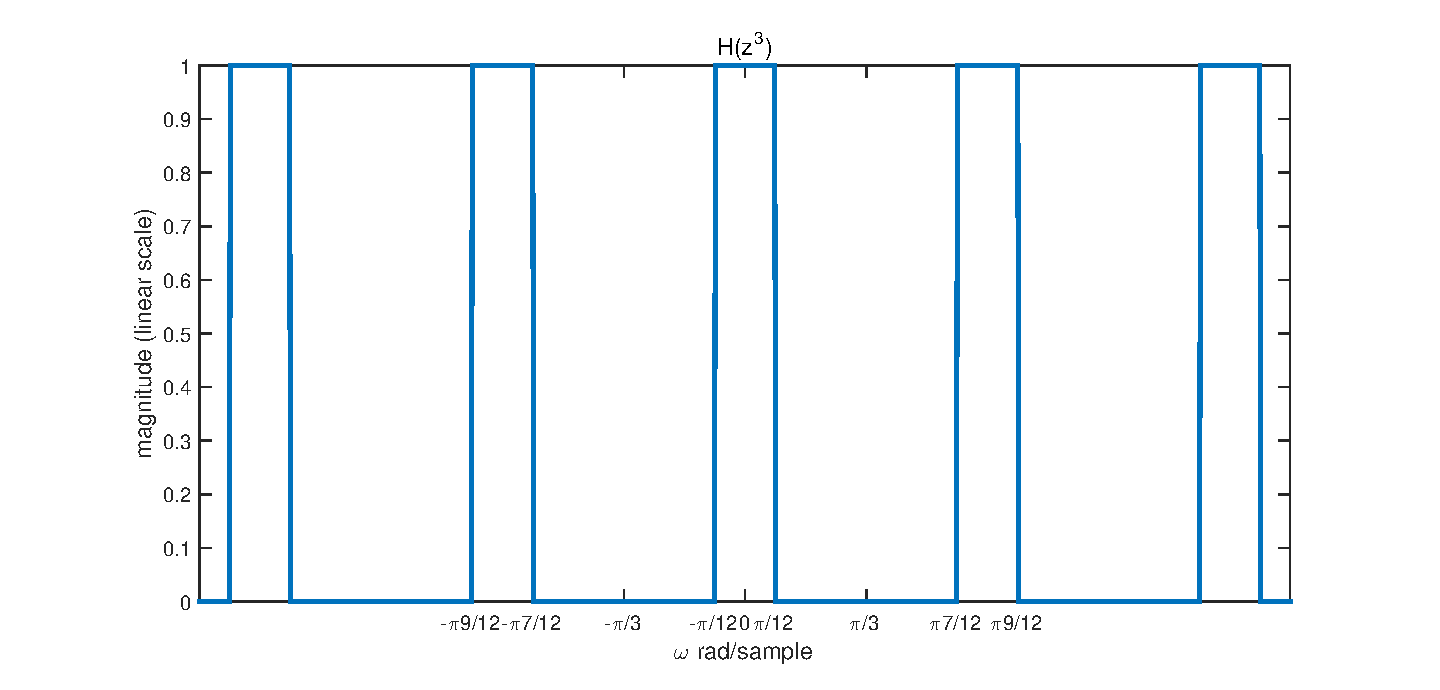
\includegraphics[width=6in]{A1bi.eps}
\caption{Magnitude response of $H(z^3)$}
\label{A1bi}
\end{figure}

\subsubsection*{(ii)}
Based on magnitude responses of $H(z)$ (Figure. \ref{A1b1}) and $H(z^3)$ (Figure. \ref{A1bi}), the product of these two can be depicted.

\begin{figure}[H]
\centering
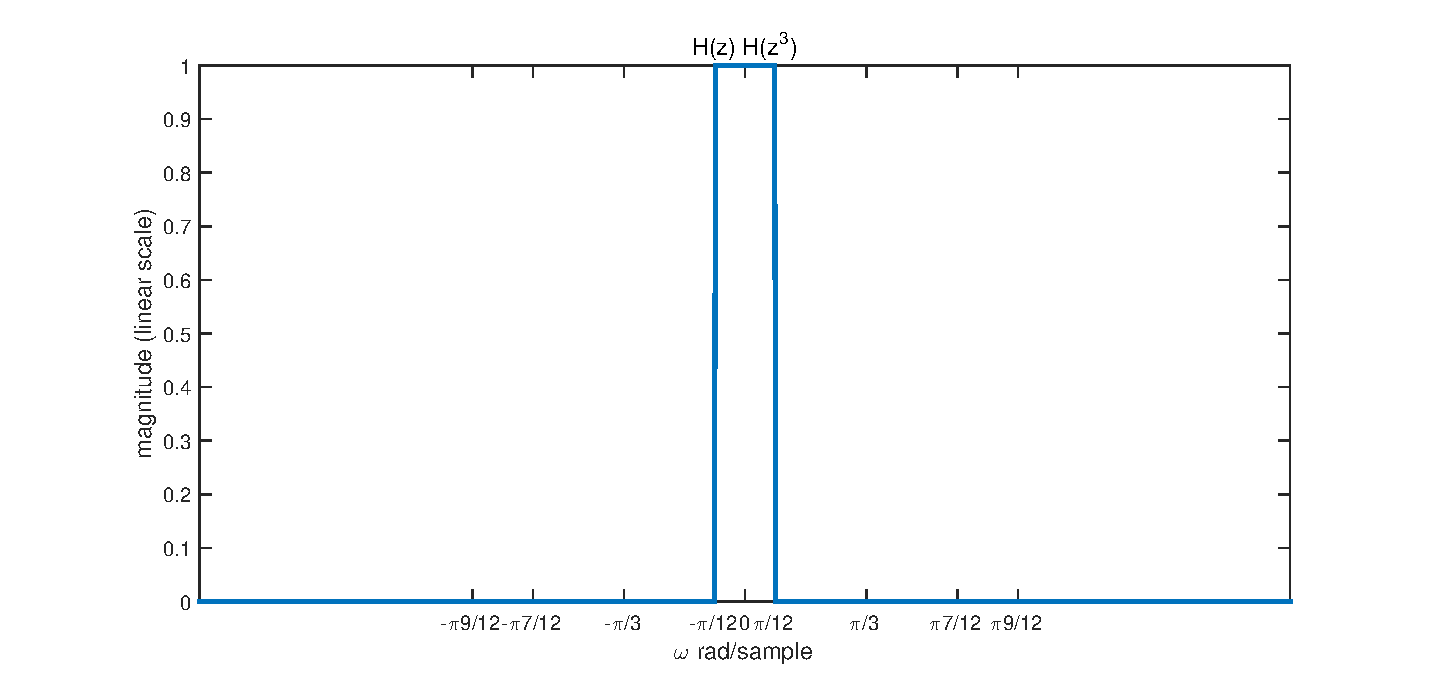
\includegraphics[width=6in]{A1bii.eps}
\caption{Magnitude response of $H(z) H(z^3)$}
\label{A1bii}
\end{figure}

\subsubsection*{(iii)}

Based on magnitude responses of $H(-z)$ (Figure. \ref{A1b2}) and $H(z^3)$ (Figure. \ref{A1bi}), the product of these two can be depicted.

\begin{figure}[H]
\centering
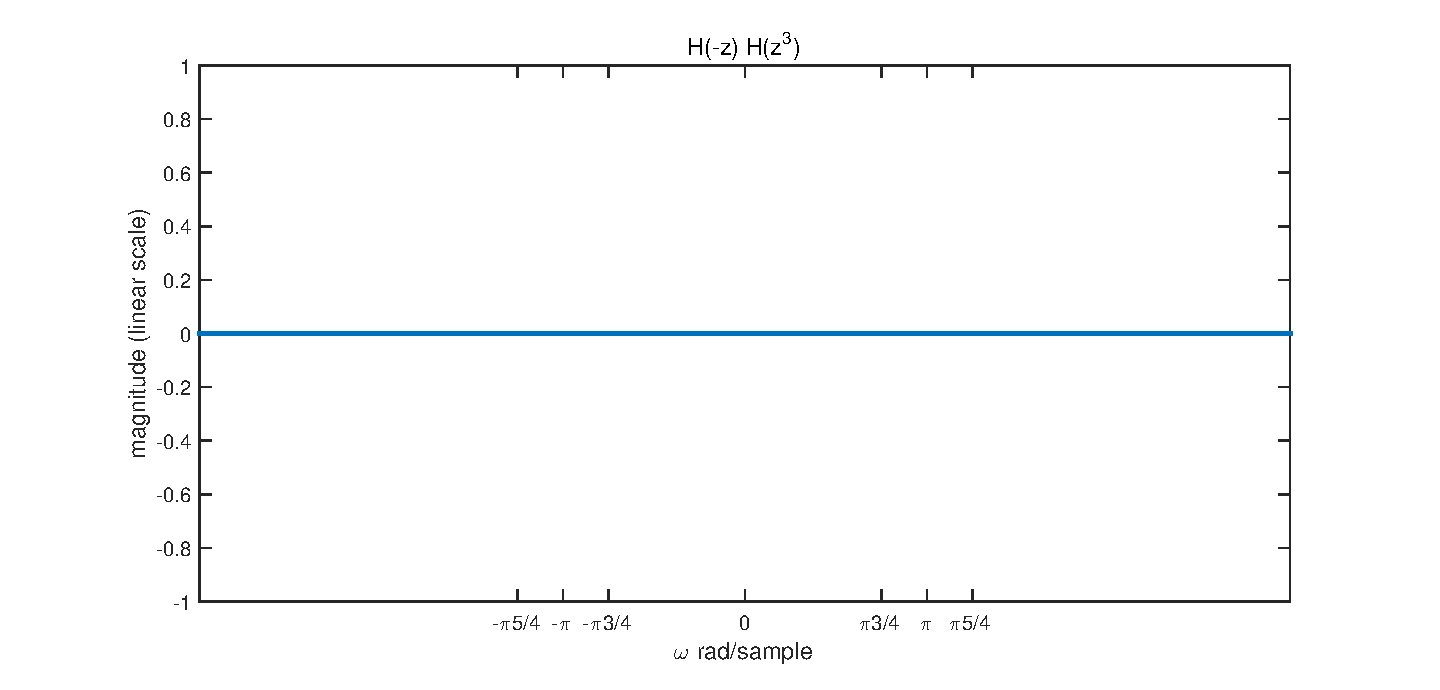
\includegraphics[width=6in]{A1biii.eps}
\caption{Magnitude response of $H(-z) H(z^3)$}
\label{A1biii}
\end{figure}

\end{homeworkSection}

\begin{homeworkSection}{c)}

Errors perhaps occur at the edge of low pass filter. For example, when $\omega = \frac{3 \pi}{4}$, $|H(-z)| = |H(z^3)| = 1$ and $|H(-z) H(z^3)| = 1$, there should be a delta impulse at $\omega = \frac{3 \pi}{4}$.

The impulse response of an ideal low pass filter:
\begin{align*}
h[n] &= \frac{1}{2\pi} \int_{-\omega_c}^{\omega_c} 1 e^{j \omega n} d\omega\\
&= \frac{1}{\pi n \times 2j} [e^{j \omega_c n} - e^{-j \omega_c n}]\\
&= \frac{\sin(\omega_c n)}{\pi n}
\end{align*}

Ideal low pass filter is impossible to be implemented in practice. $h[n]$ is infinitely long in time. It is not causal and cannot be shifted to make it causal because the impulse response extends all the way to time $-\infty$.
\end{homeworkSection}

\end{homeworkProblem}

\begin{homeworkProblem}{Question 2}

\begin{equation}\label{A21}
H_1(z) = 1 + \alpha z^{-1}
\end{equation}

\begin{homeworkSection}{a)}

\begin{equation}\label{A2a1}
H_1(z) = 1 + \alpha z^{-1} = \sum_{n=0}^{1}\alpha^{n}z^{-n}
\end{equation}

Impulse response:
\begin{equation}\label{A2a2}
h_1[n] = \sum_{i=0}^{1}\alpha^{i}\delta[n-i]
\end{equation}

Impulse response coefficients:
\begin{equation}\label{A2a3}
b_i=
\begin{cases} \alpha^i & i=0, 1\\ 0 & \text{otherwise}\\ \end{cases}
\end{equation}

\end{homeworkSection}


\begin{homeworkSection}{b)}

\begin{equation}\label{A2b1}
H_1(z^D) = 1 + \alpha z^{-D} = \frac{\alpha+z^D}{z^D}, \alpha > 0
\end{equation}

\begin{align*}
H_1(e^{j\omega D}) &= 1 + \alpha e^{-j\omega D}\\
&= 1 + \alpha \cos(\omega D) - j \alpha \sin(\omega D)\\
|H_1(e^{j\omega D})| &= \sqrt{(1 + \alpha \cos(\omega D))^2 + (\alpha \sin(\omega D))^2}\\
&= \sqrt{1 + 2 \alpha \cos(\omega D) + \alpha^2 \cos^2(\omega D) + \alpha^2 sin^2(\omega D)}\\
&= \sqrt{1 + \alpha^2 + 2 \alpha \cos(\omega D)}
\end{align*}

When $\cos(\omega D)=1$,
\begin{equation}\label{A2b2}
|H_1(e^{j\omega D})|_{max} = \sqrt{1 + \alpha^2 + 2 \alpha} = 1 + \alpha
\end{equation}
When $\cos(\omega D)=-1$
\begin{equation}\label{A2b3}
|H_1(e^{j\omega D})|_{min} = \sqrt{1 + \alpha^2 - 2 \alpha} = |1 - \alpha|\\
\end{equation}

As $|H_1(e^{j\omega D})|$ has a period of $T = \frac{2\pi}{D}$, when $\omega$ ranges in $0 \le \omega \le 2\pi$, $\frac{2\pi}{\frac{2\pi}{D}} = D$ peaks and dips occur.\\

Peaks happen at $\omega = \frac{2k\pi}{D}$ ($k=0, 1, 2, \cdots, D-1$)\\
Dips happen at $\omega = \frac{(2k+1)\pi}{D}$ ($k=0, 1, 2, \cdots, D-1$)\\

From Eq. \ref{A2b1},
\begin{align*}\label{A2b4}
1 + \alpha z^{-D} &= 0\\
z^D &= \alpha (-1)\\
&= \alpha e^{j(\pi+2k\pi)}\\
z &= \alpha^{\frac{1}{D}} e^{j\frac{(2k+1)\pi}{D}} (k = 0, 1, \cdots, D-1)
\end{align*}

\begin{figure}[H]
\begin{minipage}[t]{0.5\linewidth}
\centering
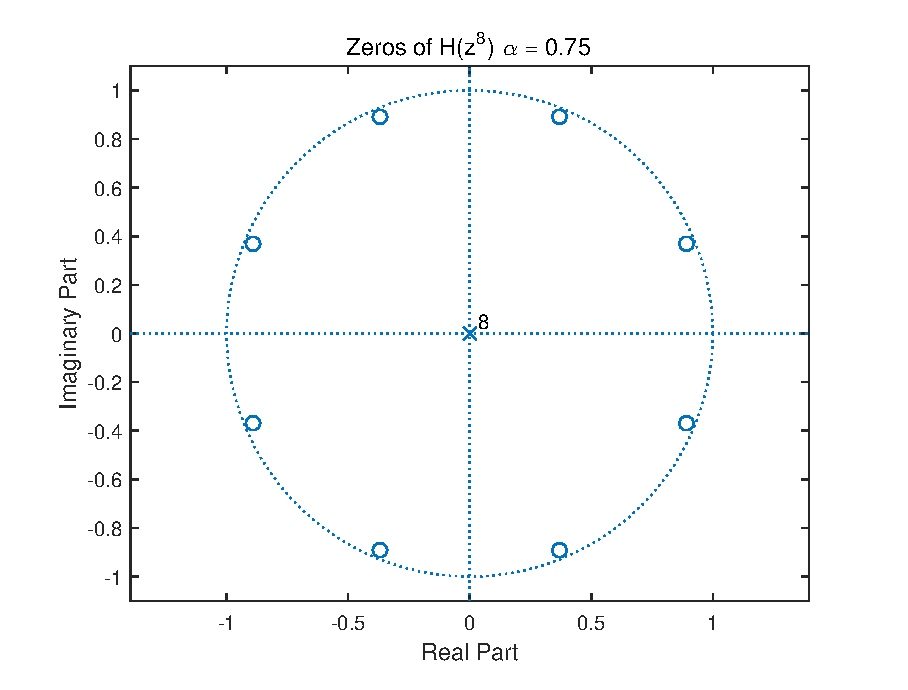
\includegraphics[width=3.3in]{A2b-zero.eps}
\caption{The zeros of the transfer function}
\label{A2b-zero}
\end{minipage}
\begin{minipage}[t]{0.5\linewidth}
\centering
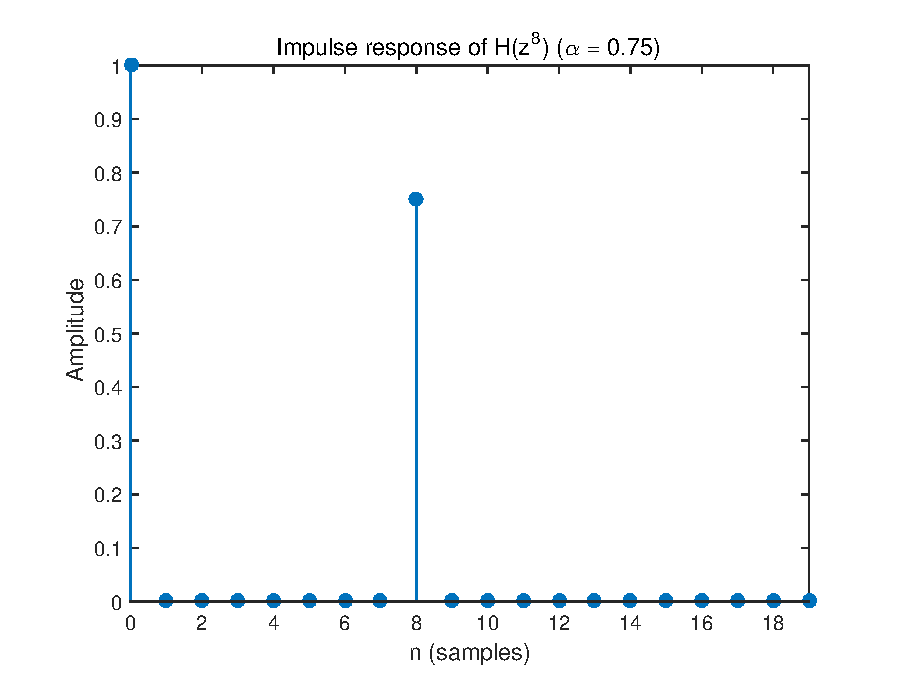
\includegraphics[width=3.3in]{A2b-impulse.eps}
\caption{The impulse response}
\label{A2b-impulse}
\end{minipage}
\end{figure}

\problemAnswer{
\vspace{5pt}
As can be seen from Figure. \ref{A2b-zero}, there are eight zeros located uniformly along a circle. Figure. \ref{A2b-impulse} shows the impulse response has horizontally stretched out 8 times (in terms of the distance between two spikes).  
}

\begin{figure}[H]
\centering
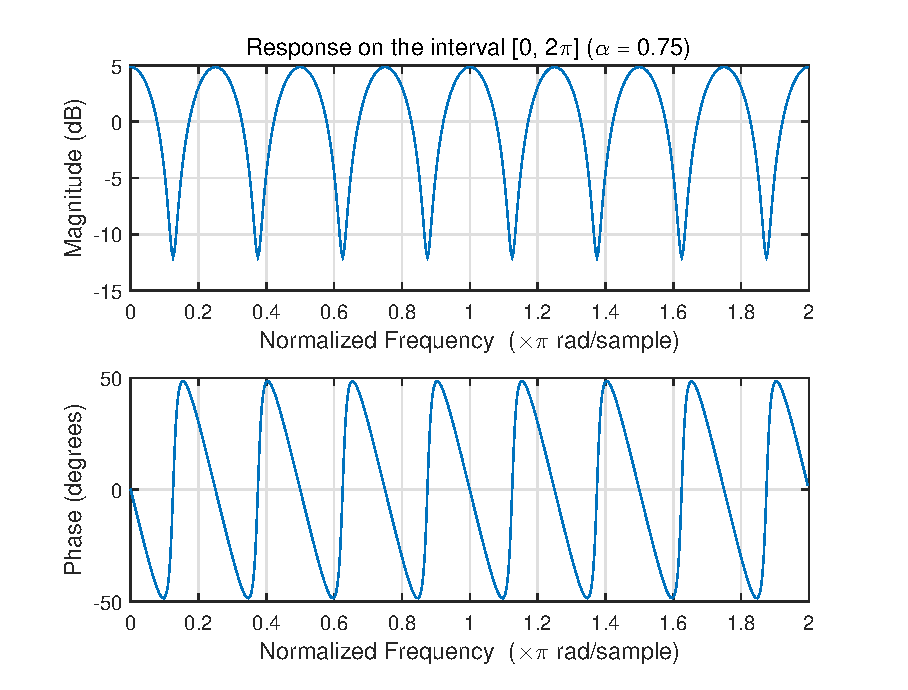
\includegraphics[width=5in]{A2b-response.eps}
\caption{The magnitude and phase response on the interval [0, $2\pi$)}
\label{A2b-response}
\end{figure}

\problemAnswer{
\vspace{5pt}
Figure. \ref{A2b-response} shows 8 peaks and 8 dips at $\frac{k\pi}{4}$ and $\frac{(2k+1)\pi}{8}$ respectively.
}

\end{homeworkSection}

\end{homeworkProblem}


\begin{homeworkProblem}{Question 3}

\begin{homeworkSection}{a)}

$H_2(z)$ is a causal filter means its inverse z transform is a right-sided sequence. If we assume the filter is stable ($|\alpha|\leq 1$), then

\begin{align*}
H_2(z) &= \frac{1}{1 + \alpha z^{-1}}\\
&= \lim_{n \to \infty} \frac{1 - (- \alpha z)^n}{1 - (- \alpha z)}\ (\text{assuming } |\alpha| < 1)\\
&= \sum_{n=0}^{\infty} (-\alpha)^n z^{-n}
\end{align*}

The region of convergence of $H_2(z)$ is exterior to a circle $|z|=|\alpha|$.\\

Frequency response:
\begin{equation*}
H_2(e^{j\omega})= \frac{1}{1 + \alpha e^{-j\omega}}
\end{equation*}

Impulse response:
\begin{equation}\label{A3a1}
h_2[n] = \sum_{i=0}^{\infty}(-\alpha)^{i}\delta[n-i]
\end{equation}

Impulse response coefficients:
\begin{equation}\label{A3a2}
b_i =
\begin{cases} (-\alpha)^i & i \ge 0\\ 0 & \text{otherwise}\\ \end{cases}
\end{equation}

\end{homeworkSection}

\begin{homeworkSection}{b)}

\begin{figure}[H]
\begin{minipage}[t]{0.5\linewidth}
\centering
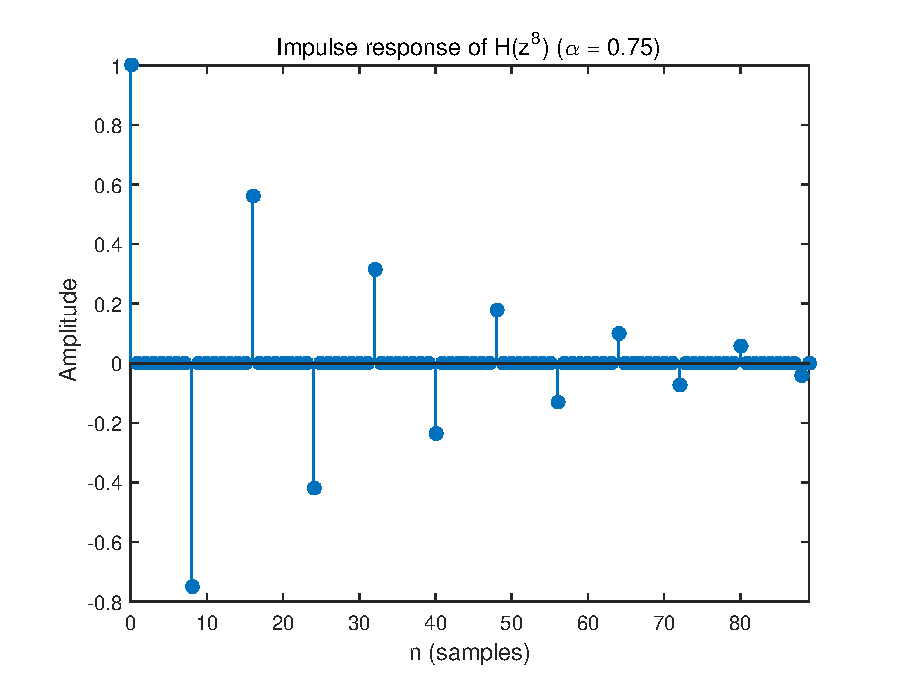
\includegraphics[width=3.3in]{A3b-impulse.eps}
\caption{The impulse response}
\label{A3b-impulse}
\end{minipage}
\begin{minipage}[t]{0.5\linewidth}
\centering
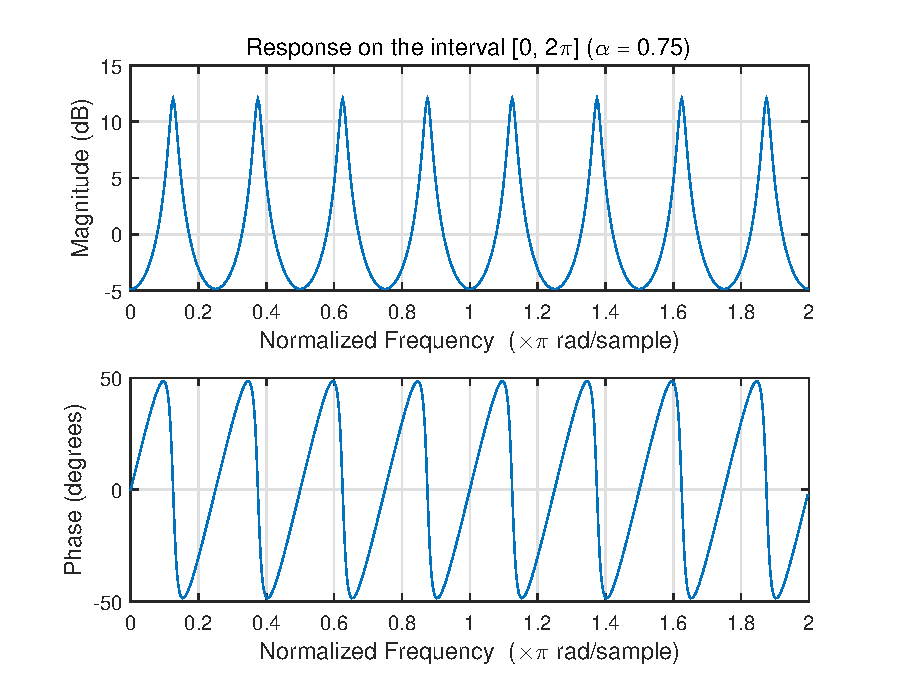
\includegraphics[width=3.3in]{A3b-response.eps}
\caption{The magnitude and phase response}
\label{A3b-response}
\end{minipage}
\end{figure}

\problemAnswer{
\vspace{5pt}
Figure. \ref{A3b-impulse} shows the impulse response of $H_2(z^8)$, the distance between any two adjacent spikes is 8. Also, the amplitude of the spike decreases as n increases (predicted by Eq. \ref{A3a2}). Figure. \ref{A3b-response} shows the magnitude and phase response in the range of $[0, 2\pi]$. 
}

\end{homeworkSection}

\end{homeworkProblem}


\begin{homeworkProblem}{Question 4}

\begin{homeworkSection}{a)}

\begin{align*}
|H_3(e^{j\omega})|^2 &=|\frac{e^{-j\omega-\alpha}}{1-\alpha e^{-j\omega}}|^2\\
&=|\frac{\cos\omega-j\sin\omega-\alpha}{1-(\alpha\cos\omega-\alpha j \sin\omega)}|^2\\
&= \frac{(\cos\omega - \alpha)^2 + (\sin\omega)^2}{(1 - \alpha\cos\omega)^2 + (\alpha\sin\omega)^2}\\
&= \frac{(\cos\omega)^2 + (\sin\omega)^2 - 2\alpha\cos\omega + \alpha^2}{1 - 2\alpha\cos\omega + \alpha^2[(\cos\omega)^2+(\sin\omega)^2]}\\
&= 1
\end{align*}

Note that $(\cos\omega)^2 + (\sin\omega)^2 = 1$.

\end{homeworkSection}

\begin{homeworkSection}{b)}

First define
\begin{equation}\label{A4a}
h_0[n] = \begin{cases} (\alpha)^n & n \in \mathbb{N} \\ 0 & \text{otherwise}\\ \end{cases}
\end{equation}

Take the z-transform
\begin{equation}\label{A4b}
H_0(z)=\sum_{n=0}^{\infty}h_0[n] z^{-n}=\sum_{n=0}^{\infty}(\alpha)^n z^{-n}
\end{equation}

\begin{align*}
H_3(z)&=\frac{z^{-1}-\alpha}{1-\alpha z^{-1}}\\
&=\frac{z^{-1}}{1-\alpha z^{-1}}-\frac{\alpha}{1-\alpha z^{-1}}\\
&=z^{-1}\sum_{n=0}^{\infty}(\alpha)^n z^{-n}-\alpha\sum_{n=0}^{\infty}(\alpha)^n z^{-n}\\
&=z^{-1} H_0(z) - \alpha H_0(z)
\end{align*}
Take inverse z transform on both sides and apply time shift and linearity property,
\begin{align*}
h_3[n] &= h_0[n-1] - \alpha h_0[n] = \alpha^{n-1} - \alpha \cdot \alpha^n = (1-\alpha^2) \alpha^{n-1} \text{ (for $n>0$)}
\end{align*}

Since the filter is causal, $h_3[n]=0$ for $n<0$.\\

When $n=0$, $h_3[0] = h_0[-1] - \alpha h_0[0] = -\alpha h_0[0] = -\alpha$.

\end{homeworkSection}

\begin{homeworkSection}{c)}

\begin{figure}[H]
\begin{minipage}[t]{0.5\linewidth}
\centering
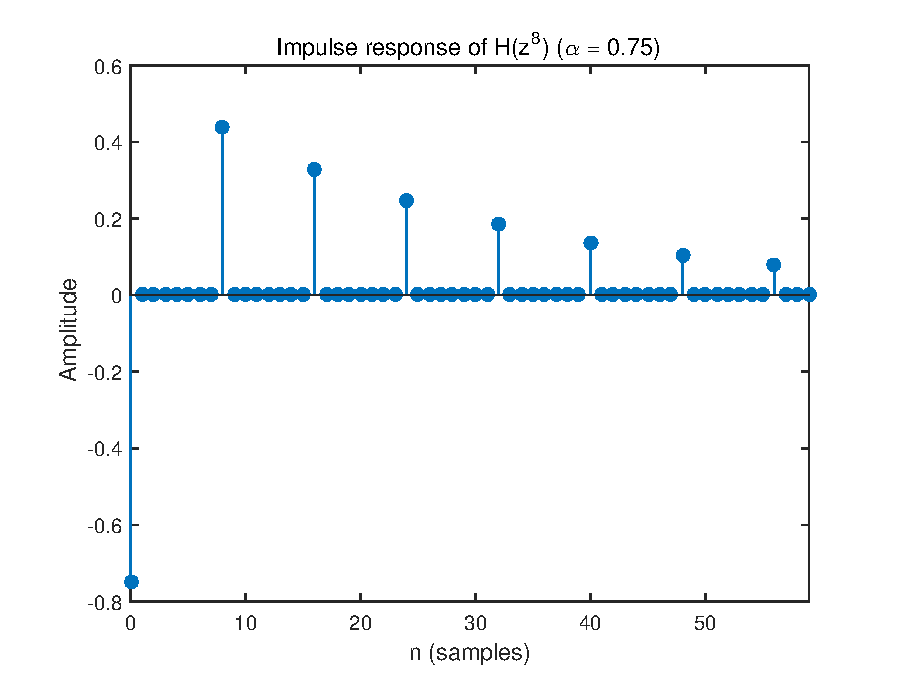
\includegraphics[width=3.3in]{A4c-impulse.eps}
\caption{The impulse response}
\label{A4c-impulse}
\end{minipage}
\begin{minipage}[t]{0.5\linewidth}
\centering
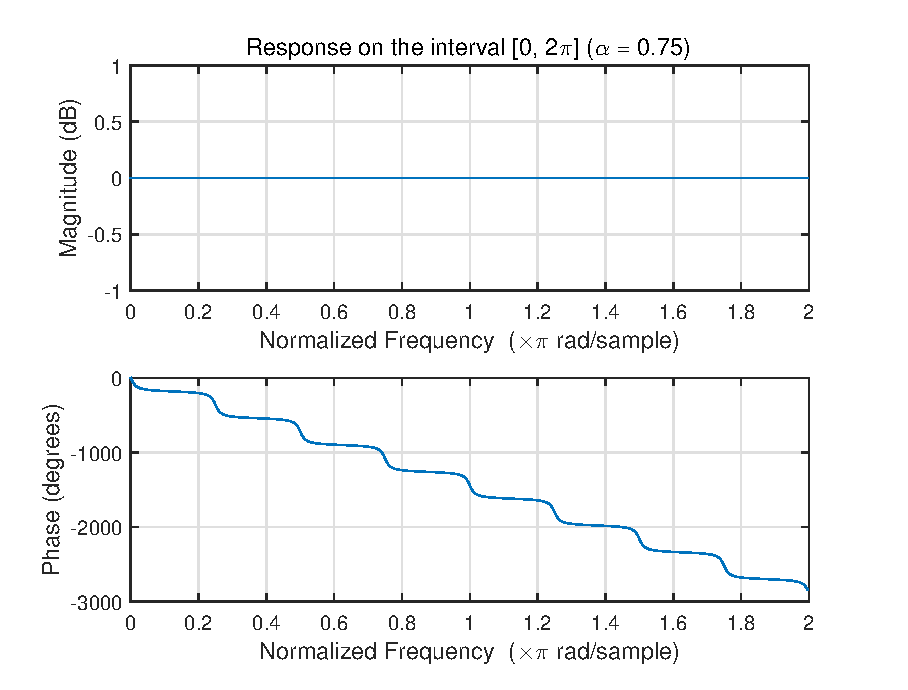
\includegraphics[width=3.3in]{A4c-response.eps}
\caption{The magnitude and phase response}
\label{A4c-response}
\end{minipage}
\end{figure}

\end{homeworkSection}

\end{homeworkProblem}


\begin{homeworkProblem}{Question 5}

\begin{equation}\label{A51}
\omega_0 = \frac{2\pi \times 330 \text{ Hz}}{44.1 \times 10^3 \text{ sample/s}} = 0.04701 \text{ rad/sample}
\end{equation}

\begin{equation}\label{A52}
H_{BS}(z) = \frac{1+\alpha}{2} \frac{1-2\beta z^{-1} + z^{-2}}{1 - \beta (1+\alpha) z^{-1} + \alpha z^{-2}}
\end{equation}
where $\beta = \cos(\omega_0) = \textbf{0.9989}$.\\

Poles at $r e^{\pm j\phi}$, a stable system requires $r=\sqrt{\alpha}<1$, i.e. $0<\alpha<1$.

\begin{equation}\label{A53}
B_w = \cos^{-1}(\frac{2\alpha}{1+\alpha^2})\\
\end{equation}

Given $0<\alpha<1$
\begin{equation}\label{A54}
\alpha = \frac{1}{\cos(B_w)} - \sqrt{\frac{1}{(\cos(B_w))^2}-1}
\end{equation}

\begin{homeworkSection}{(i) $B_w = 0.1\pi$}

When $B_w = 0.1\pi$, from Eq. \ref{A54}
\begin{equation}
\alpha = 0.726543
\end{equation}

\begin{figure}[H]
\begin{minipage}[t]{0.5\linewidth}
\centering
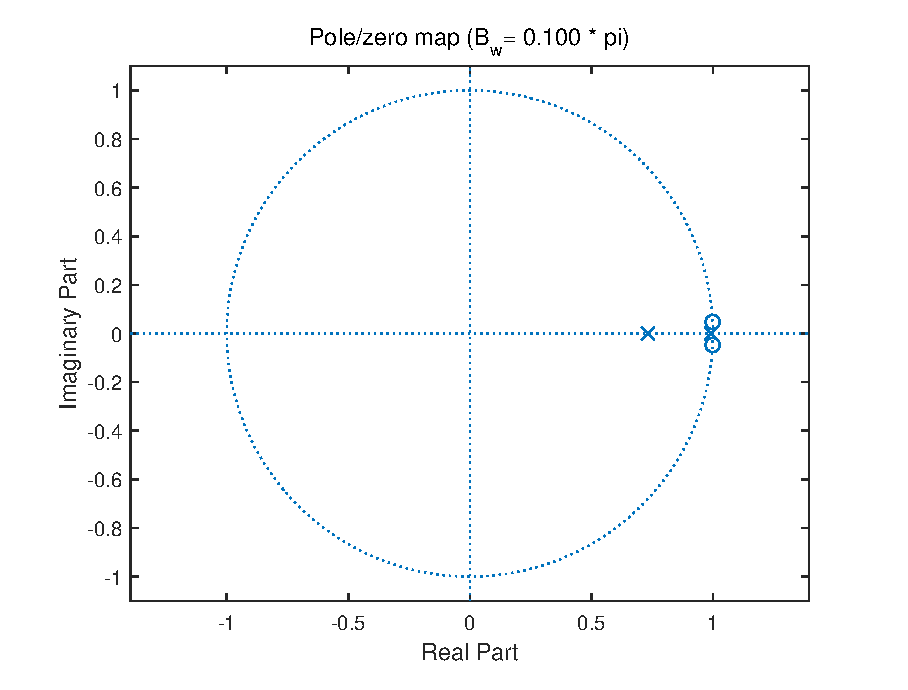
\includegraphics[width=3.3in]{A5i-pole.eps}
\caption{The pole / zero map}
\label{A5i-pole}
\end{minipage}
\begin{minipage}[t]{0.5\linewidth}
\centering
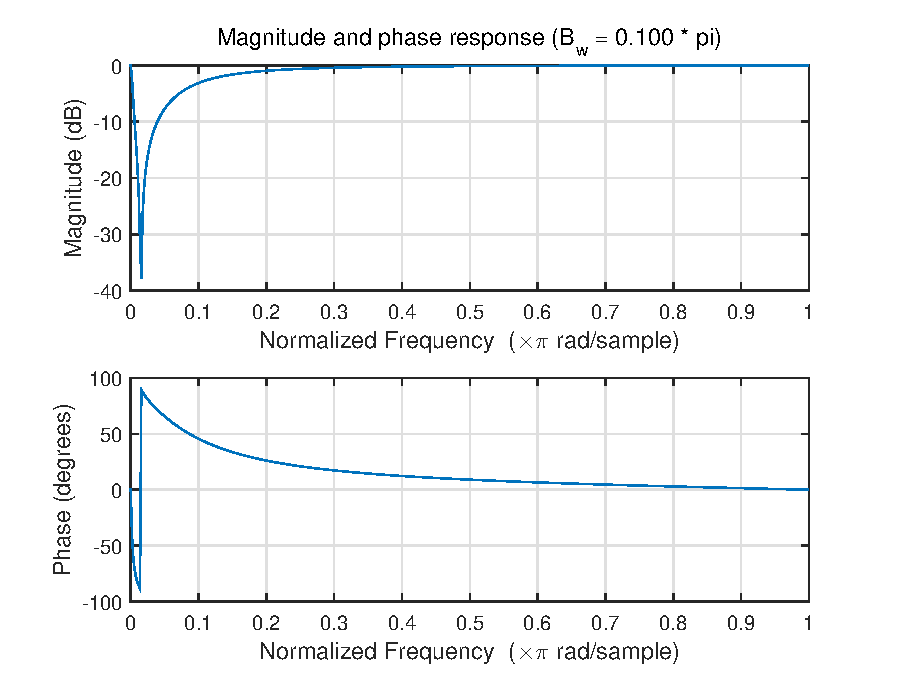
\includegraphics[width=3.3in]{A5i-response.eps}
\caption{The magnitude and phase response}
\label{A5i-response}
\end{minipage}
\end{figure}

\end{homeworkSection}

\begin{homeworkSection}{(ii) $B_w = 0.01\pi$}

When $B_w = 0.01\pi$, from Eq. \ref{A54}
\begin{equation}
\alpha = 0.969067
\end{equation}

\begin{figure}[H]
\begin{minipage}[t]{0.5\linewidth}
\centering
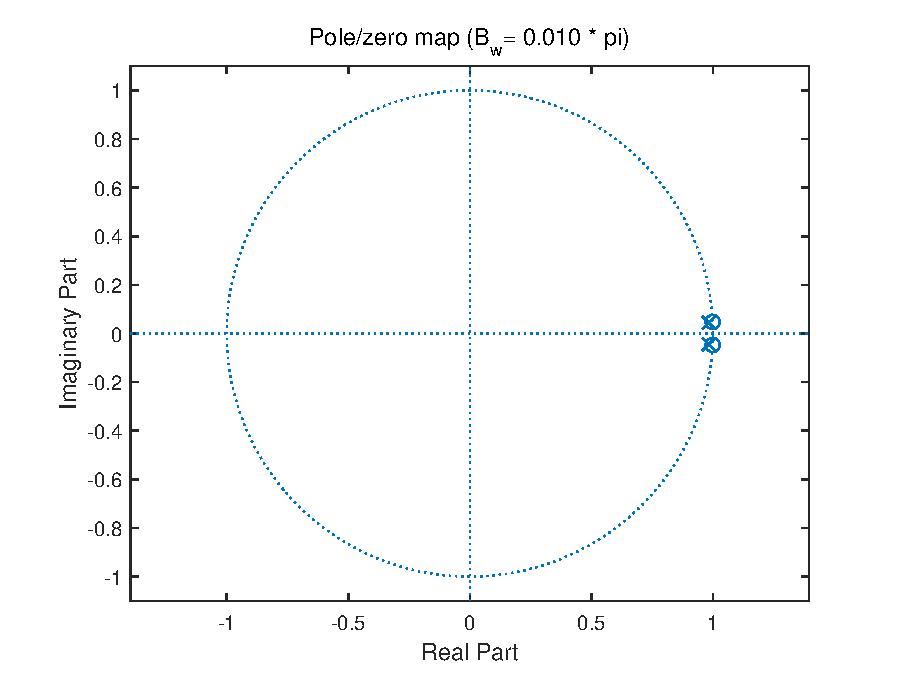
\includegraphics[width=3.3in]{A5ii-pole.eps}
\caption{The pole / zero map}
\label{A5ii-pole}
\end{minipage}
\begin{minipage}[t]{0.5\linewidth}
\centering
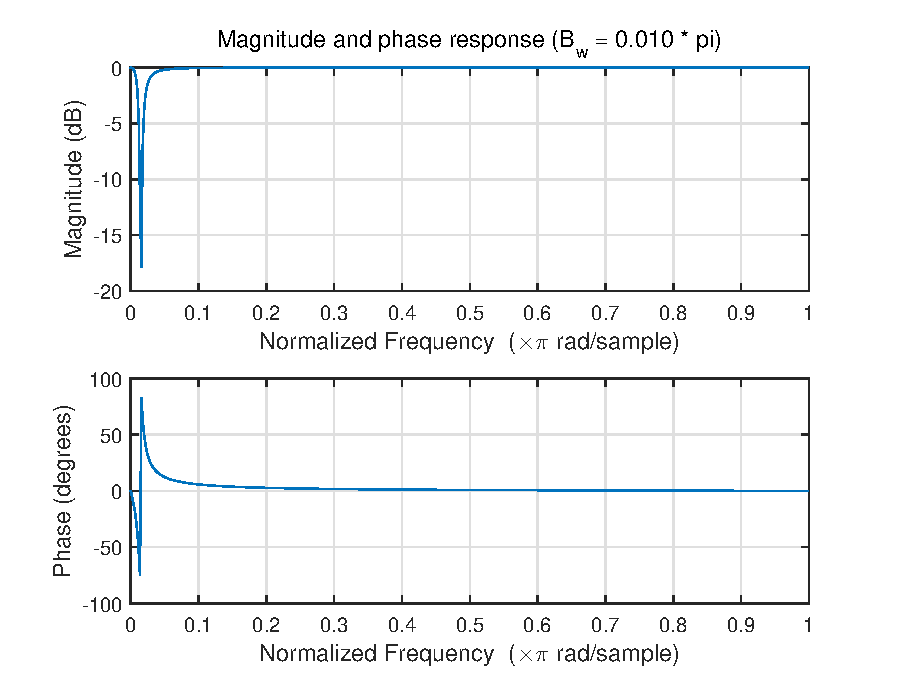
\includegraphics[width=3.3in]{A5ii-response.eps}
\caption{The magnitude and phase response}
\label{A5ii-response}
\end{minipage}
\end{figure}

\end{homeworkSection}

\begin{homeworkSection}{(iii) $B_w = 0.005\pi$}

When $B_w = 0.005\pi$, from Eq. \ref{A54}
\begin{equation}
\alpha = 0.984414
\end{equation}

\begin{figure}[H]
\begin{minipage}[t]{0.5\linewidth}
\centering
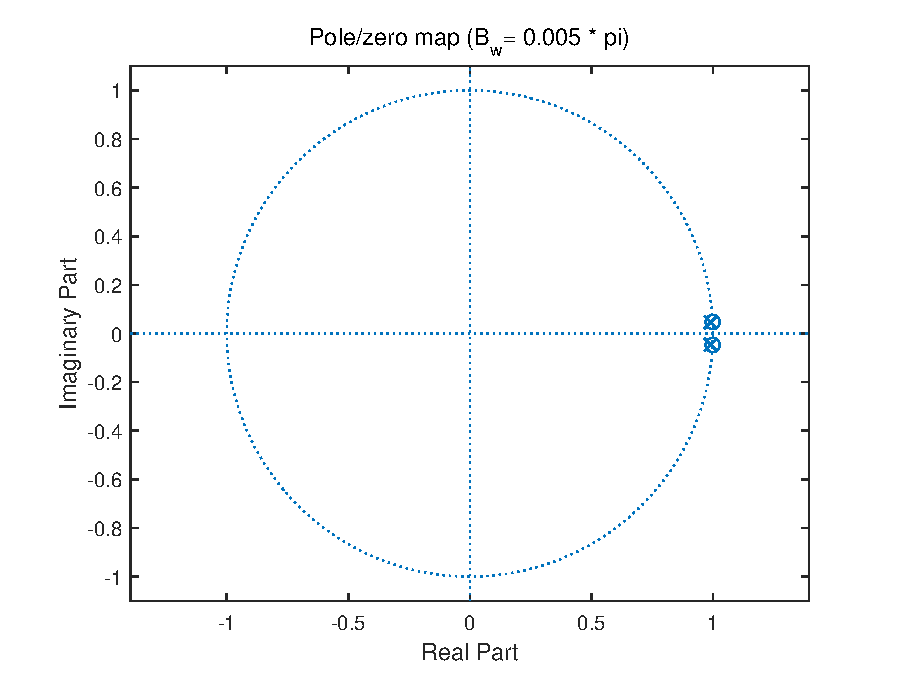
\includegraphics[width=3.3in]{A5iii-pole.eps}
\caption{The pole / zero map}
\label{A5iii-pole}
\end{minipage}
\begin{minipage}[t]{0.5\linewidth}
\centering
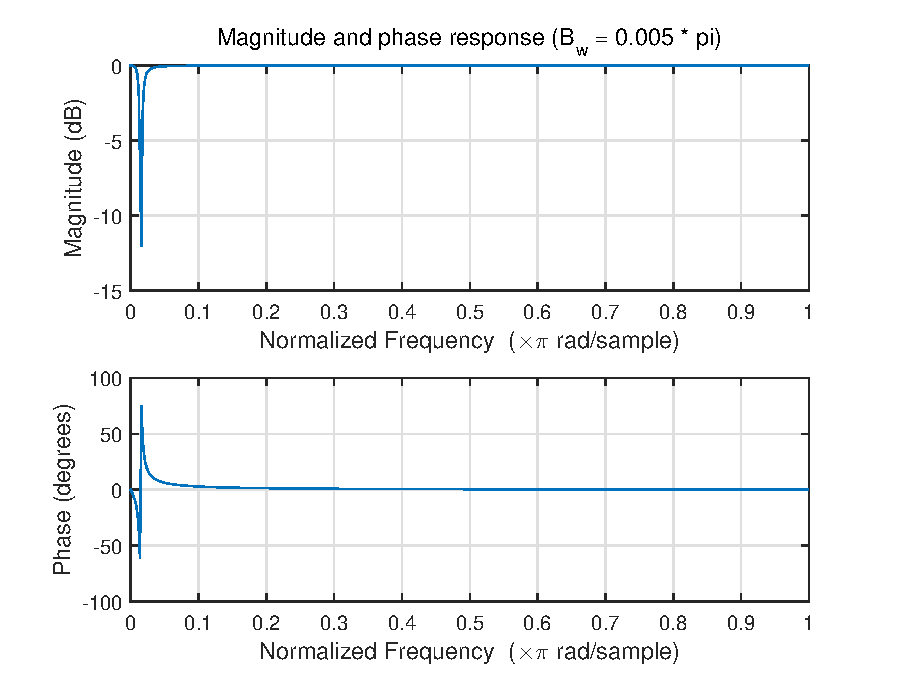
\includegraphics[width=3.3in]{A5iii-response.eps}
\caption{The magnitude and phase response}
\label{A5iii-response}
\end{minipage}
\end{figure}

\end{homeworkSection}

\problemAnswer{
As the bandwidth is reduced, the notch filter will more concentrate on the specific frequency, in other words, rejective band becomes narrower. However, poles go closer to zeros and the unit circle, which makes it hard to stabilize the filter system.
}

\begin{homeworkSection}{MATLAB function}
\problemAnswer{
	\lstinputlisting{A5_function.m}
}
\end{homeworkSection}

\end{homeworkProblem}


%----------------------------------------------------------------------------------------
%	Appendix
%----------------------------------------------------------------------------------------

\newpage
\begin{homeworkProblem}{Appendix}

\begin{homeworkSection}{Question 1 b)}
	\lstinputlisting{A1b.m}
\end{homeworkSection}

\begin{homeworkSection}{Question 2 b)}
	\lstinputlisting{A2b.m}
\end{homeworkSection}

\newpage
\begin{homeworkSection}{Question 3 b)}
	\lstinputlisting{A3b.m}
\end{homeworkSection}

\begin{homeworkSection}{Question 4 c)}
	\lstinputlisting{A4c.m}
\end{homeworkSection}

\newpage
\begin{homeworkSection}{Question 5 plot}
	\lstinputlisting{A5_plot.m}
\end{homeworkSection}

\begin{homeworkSection}{Question 5 sound}
	\lstinputlisting{A5_sound.m}
\end{homeworkSection}

\end{homeworkProblem}

%----------------------------------------------------------------------------------------

\end{document}
